\section{Design Overview}\label{s:design}

\begin{figure*}
    \centering
    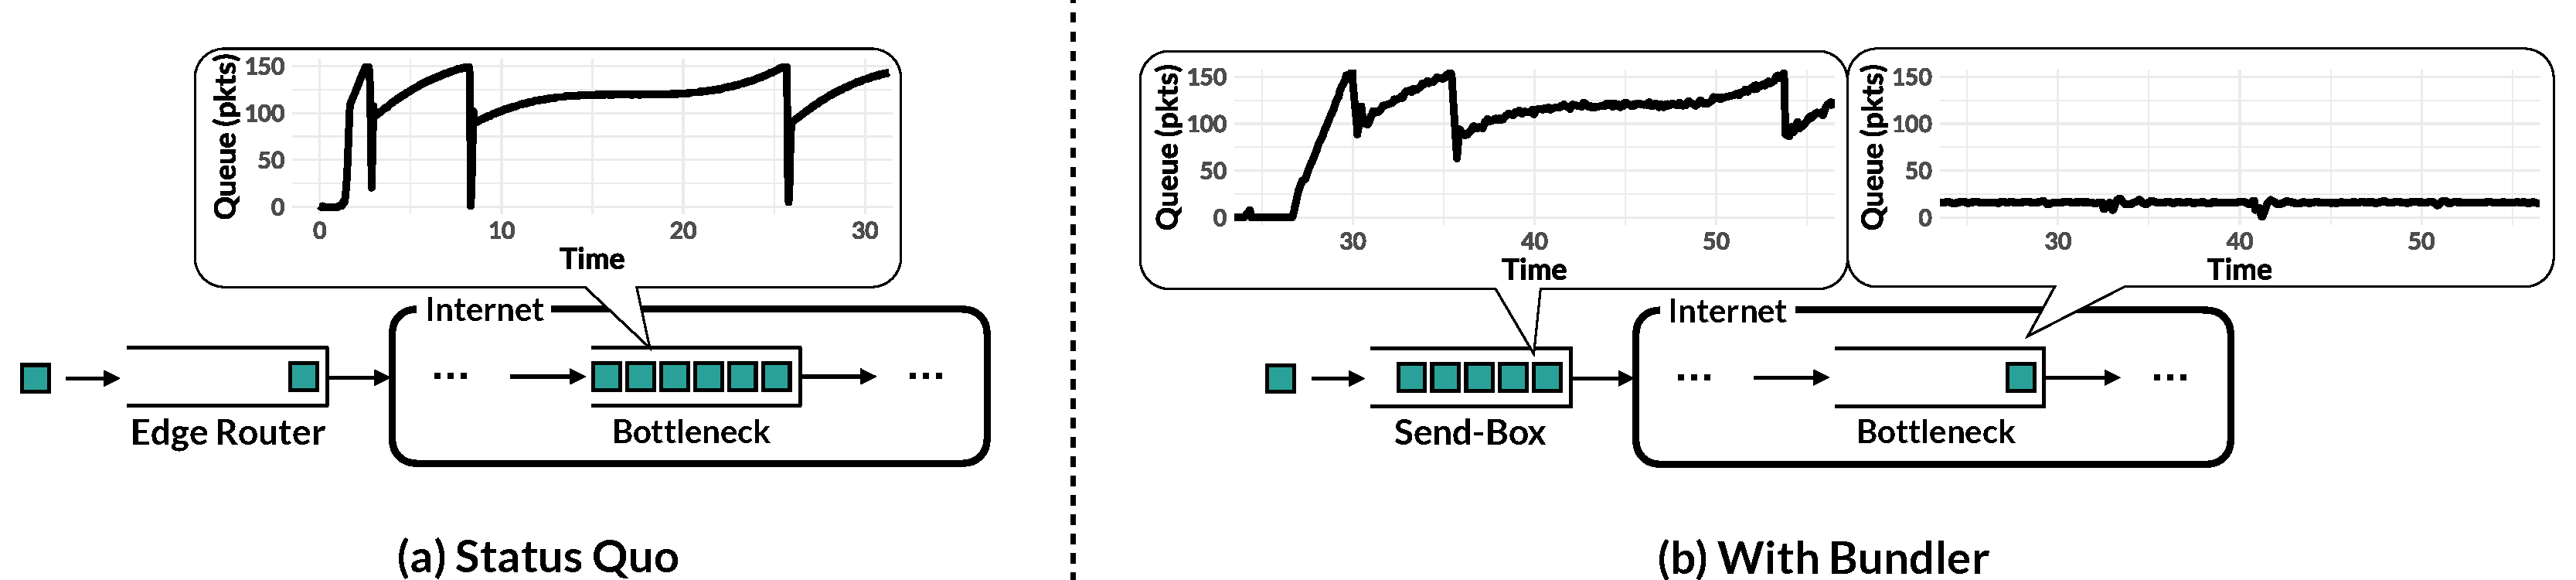
\includegraphics[width=\textwidth]{img/shift-bottleneck-combined}
    \caption{This illustrative example with a single flow shows how \name can take control of queues in the network. The plots show the trend in measured queueing delays at the relevant queue over time. The queue where delays build up can best make scheduling decisions, since it has the most choice between packets to send. Therefore, the \inbox \emph{shifts} the queues to itself to gain scheduling power.}\label{fig:design:shift-bottleneck}
\end{figure*}

Recall that in order to do scheduling, we need to move the queues from the network to the \name. 
In this section, we first describe our key insight for moving the in-network queues, and then explain our specific design choices. 

\subsection{Key Insight}
A trivial strategy for inducing queuing at the \name is to throttle its outgoing rate. However, if this rate is made smaller than the bundle's share of bandwidth at the bottleneck link in the network, it can decrease throughput. Instead, the rate needs to be set such that the bottleneck link sees a small queue while remaining fully utilized (and the bundled traffic competes fairly in the presence of cross traffic). 
We make a simple, but powerful, observation: existing congestion control algorithms perform exactly this calculation~\cite{Jacobson88}. 
Therefore, running such an algorithm at the \inbox to set a bundle's rate would reduce its self-inflicted queue at the bottleneck, shifting it to the \inbox instead, without impacting aggregate throughput. 
Note that each end host would continue running a traditional congestion control algorithm (\eg Cubic~\cite{cubic}, BBR~\cite{bbr}), as before, which is unaware of \name, but build queues at \inbox rather than in the network.

Figure~\ref{fig:design:shift-bottleneck} illustrates this concept for a single flow traversing a bottleneck link in the network.
\footnote{Details of the emulated network setup which resulted in the illustrated queue length time-series are in \S\ref{s:eval}.} 
Without \name, packets from the end hosts are queued in the network, while the queue at the edge is unoccupied. 
In contrast, a \name deployed at the edge is able to shift the queue to its \inbox.

\subsection{Design Choices}

Our key requirement of \emph{deployment and management ease} guides our design choices:

\paragraphn{(i)} \name requires no changes to the endhosts or to the routers in the network, making it independently deployable. 

\paragraphn{(ii)} \name maintains only per-bundle state, and no per-connection state (unless needed by a specific scheduling algorithm), allowing it to scale trivially with the number of in-bundle connections. 

\paragraphn{(iii)} The only persistent state maintained in the \name is the network condition (in the form of congestion signals) which can be naturally re-aquired, thus making it crash-resistant. 

\paragraphn{(iv)} \name supports an entirely passive deployment model in which its component packets remain unmodified, 
ensuring no interference with other networking components in a packet's path~\cite{mboxbadness, ipoptions, quic}. We discuss this further in \an{forward pointer}.

\vspace{5pt}
\noindent We discuss specific design choices in more details below. 

\subsubsection{Choice of congestion control algorithm}
\name's congestion control algorithm must satisfy the following requirements: 

\paragraphi{(1) Ability to limit network queueing} \name must limit queueing in the network to move the queues to the \inbox. Therefore, congestion control algorithms which are designed to control delays are the appropriate choice. 
A window-probing congestion control algorithm, for example, is not a good choice for \name, since it would build up a queue at the network bottleneck and drain queues at the \inbox.

\paragraphi{(2) Detection of buffer-filling cross-traffic} Simultaneously, it is well-known that delay-controlling schemes (\eg Vegas~\cite{vegas}) compete poorly with buffer-filling window-probing schemes, since buffer occupancy determines throughput fairness~\cite{Jacobson88}. 
Therefore, \name must have a mechanism to detect the presence of such competing buffer-filling flows, and fall back to status quo performance (we discuss the mechanism for falling back to status quo performance in \S\ref{s:queue-ctl}).

The emergence of such detection mechanisms is recent: Copa~\cite{copa} detects whether the queue lengths it observes are consistent with its own fluctuations, and Nimbus\footnote{Nimbus is descibed in concurrently submitted work: paper \an{XX}} provides a more general mechanism which overlays a pattern on the sending rate and measures the cross traffic's response.
\name uses the Nimbus detection mechanism and can use any delay-controlling algorithm, as shown in Figure~\ref{fig:eval:cc}.

\subsubsection{Two-sided measurement of congestion signals}\label{s:design:twosided}
Congestion control algorithms require network feedback from the receivers to measure congestion and adjust the sending rates accordingly. 
Conventional endhost-based implementations have used TCP acknowledgements for this.
However, this is not a good option for \name because: 
(i) it is specific to TCP and thus incompatible with alternate protocols, \ie UDP for video streaming or QUIC's encrypted transport header~\cite{quic}, 
and (ii) it requires the reverse traffic to also pass through \name's \inbox, which may not always be the case.  

This problem presents multiple possible solutions:

\paragrapha{Terminate connections and proxy through TCP} This approach allows the unmodified use of existing congestion control algorithms, since a TCP tunnel can collect ACKs. Furthermore, TCP proxies can improve performance by allowing end-to-end connections to ramp up their sending rates quickly.
The primary disadvantage of this approach is that \name must take responsibility for reliable delivery of component traffic, which in the case of UDP applications can harm application performance. 
Indeed, from an architectural standpoint, this design runs counter to the end-to-end principle~\cite{e2e-principle}; it replicates endhost functionality in the network.
Furthermore, from a practical standpoint, to avoid head-of-line blocking this approach requires that \name open a new proxy connection for each component end-host connection, but still determine the bottleneck rate of the traffic \emph{aggregate}. While this approach may be technically feasible~\cite{cm}, opening and managing new proxy connections may use cycles better used for packet processing.
Thus, we set aside TCP tunnels for the remainder of this discussion, but note that this approach is complementary with \name (see \S\ref{s:eval}).

Despite the shortcomings of TCP tunnels, the core idea of tunnelling to support new functionality is sound~\cite{trotsky}; we simply note that it is advantageous for the tunnels to be unreliable. We thus adopt unreliable tunnelling in \name.

\paragrapha{Unreliable tunnelling mechanisms and congestion ACKs} Protocols at both L3 (\eg NVGRE~\cite{nvgre}, IP-in-IP~\cite{ipinip}) and L4 (\eg VXLAN~\cite{vxlan}) are broadly avaiable and deployed in commodity routers today. We further envision an even simpler case: a ``null'' tunnel, where packets pass through the \inbox entirely unmodified.
In these two cases, there is no natural stream of returning TCP ACKs with which to measure congestion information. 
Rather, \name uses congestion-specific ACKs\footnote{The idea of a congestion ACK is similar to that in QCN~\cite{qcn}, although our goals differ.} via a two-sided design, with the following properties:

\paragraphi{(1) Out-of-band feedback} 
The \outbox sends explicit out-of-band \emph{feedback messages} to the \inbox, which are used for measuring congestion signals. 
This out-of-band feedback mechanism is not only agnostic to the underlying protocol (be it TCP or UDP), but also side-steps the issue of enforcing that TCP acknowledgements pass through the same \inbox.

\paragraphi{(2) Infrequent measurements} Sending an out-of-band feedback message for every packet arriving at the \outbox would result in high communication overhead. Furthermore, conducting measurements on every outgoing packet at the \inbox would require maintaining state for each of them, which can be expensive, especially at high bandwidth-delay products. We, therefore, conduct measurements on a few sampled packets, at least once per RTT, which is sufficient for most congestion control algorithms~\cite{ccp}. 

We detail two-sided congestion measurements in \S\ref{s:measurement}.
